\documentclass[tikz,border=2pt]{standalone}
\usepackage{amsmath,amssymb}
\usepackage{pgfplots}
\pgfplotsset{compat=1.18}

\begin{document}
% A two-component normal mixture: with probability 0.4 draw from N(-1.5, 0.6^2), otherwise
% from N(1.5, 0.8^2); the mixture density is the weighted average of the two.
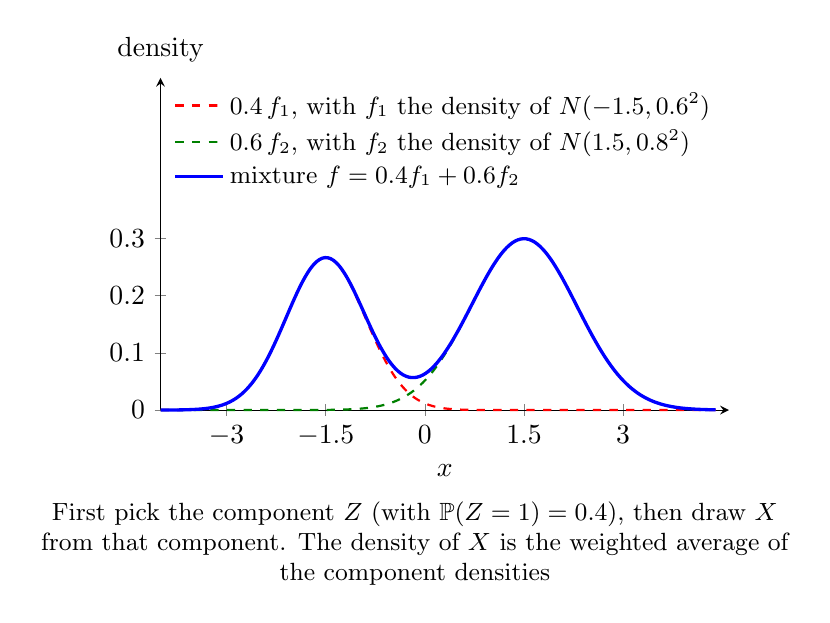
\begin{tikzpicture}
	\begin{axis}[
		axis lines=left, xmin=-4, xmax=4.6, ymin=0, ymax=0.58,
		xtick={-3,-1.5,0,1.5,3}, ytick={0,0.1,0.2,0.3},
		xlabel={$x$}, ylabel={density}, ylabel style={rotate=-90, anchor=south, at={(axis description cs:0,1.02)}},
		samples=200, smooth, width=8.8cm, height=5.8cm, clip=false,
		legend style={draw=none, fill=none, font=\small, at={(0.5,0.99)}, anchor=north}, legend cell align=left
		]
		\addplot[red, thick, dashed, domain=-4:4.4] {0.4*exp(-(x+1.5)^2/(2*0.36))/(0.6*sqrt(2*pi))};
		\addlegendentry{$0.4\,f_1$, with $f_1$ the density of $N(-1.5,0.6^2)$}
		\addplot[green!50!black, thick, dashed, domain=-4:4.4] {0.6*exp(-(x-1.5)^2/(2*0.64))/(0.8*sqrt(2*pi))};
		\addlegendentry{$0.6\,f_2$, with $f_2$ the density of $N(1.5,0.8^2)$}
		\addplot[blue, very thick, domain=-4:4.4] {0.4*exp(-(x+1.5)^2/(2*0.36))/(0.6*sqrt(2*pi))+0.6*exp(-(x-1.5)^2/(2*0.64))/(0.8*sqrt(2*pi))};
		\addlegendentry{mixture $f=0.4f_1+0.6f_2$}
	\end{axis}
	\node[anchor=north, font=\small, align=flush center, text width=9.6cm] at ([yshift=-2pt]current axis.outer south) {First pick the component $Z$ (with $\mathbb{P}(Z=1)=0.4$), then draw $X$ from that component. The density of $X$ is the weighted average of the component densities};
\end{tikzpicture}
\end{document}
